% DMRN+21: the official 2026 kit ships the 2025 style; its event header and
% footer are updated in the local copy, without changing its page layout.
\documentclass[a4paper]{article}
\usepackage[T1]{fontenc}
\usepackage{caption}
\usepackage{times,amsmath,graphicx,url,dmrn2026}
\usepackage{indentfirst}
\usepackage{xcolor}
\captionsetup[figure]{skip=2pt}\setlength{\intextsep}{3pt plus 1pt minus 1pt}
\setlength{\parskip}{0.1em}
\captionsetup[figure]{font=footnotesize,labelfont=footnotesize}
\captionsetup[table]{font=footnotesize,labelfont=footnotesize}
\setlength{\belowcaptionskip}{0pt}
\renewcommand{\thesection}{\Roman{section}}
\newcommand{\head}[1]{\par\vspace{1pt}\noindent\textbf{#1.}\ \ignorespaces}
% Tighter display spacing. \ninept makes \normalsize an alias of \small, which
% resets the display skips at every size switch, so the reduced values are
% appended to \small itself.
\makeatletter
\g@addto@macro\small{\abovedisplayskip 4pt plus 1pt minus 1pt \belowdisplayskip 4pt plus 1pt minus 1pt
 \abovedisplayshortskip 2pt \belowdisplayshortskip 2pt plus 1pt}
\makeatother
\providecommand{\bstctlentry}[1]{\nocite{#1}}
% No extra space between reference entries.
\let\oldthebibliography\thebibliography
\renewcommand{\thebibliography}[1]{\oldthebibliography{#1}\setlength{\itemsep}{0pt}\setlength{\parskip}{0pt}}
% Layout economies after the DMRN+15 auraloss one-pager: tighter title block,
% 7 pt footer close to the page edge, taller text block. The style file is unchanged.
\setlength{\textheight}{266truemm}\setlength{\footskip}{0.2in}
\cfoot{\fontsize{7}{8}\selectfont\textsc{DMRN+21: DIGITAL MUSIC RESEARCH NETWORK ONE-DAY WORKSHOP 2026, KING'S COLLEGE LONDON, FRI 11 DECEMBER 2026}}
\makeatletter
\def\@maketitle{\newpage
 \null
 \begin{minipage}{0.5\textwidth}
 \textsc{DMRN+21: Digital Music Research Network\\One-day Workshop 2026}\vspace{3mm}\\\textsc{King's College London}\\\textsc{Fri 11 December 2026}
 \end{minipage}%
 \begin{minipage}{0.5\textwidth}
 \hfill\hbox{
\includegraphics[width=6cm]{DMRN_Logo_high_res.jpg}}
 \end{minipage}
 \vskip 0.4em \begin{center}
 {\large \bf \@title \par} \vskip 0.35em {\large
\begin{tabular}[t]{c}\@name \\ \@address
 \end{tabular}
 \par}
 \end{center}
 \par
 \vskip 0.2em}
\makeatother

\title{Efficient Backprop for an FDTD Kirchhoff--Carrier String}
\name{\normalfont Pablo Tablas de Paula, Emmanouil D. Benetos and Joshua D. Reiss\thanks{This work was supported by UKRI grant EP/S022694.}}
\address{\small Centre for Digital Music, Queen Mary University of London, p.tablasdepaula@qmul.ac.uk}

\begin{document}
\bstctlentry{BSTcontrol}
\ninept
\maketitle
\begin{sloppy}
\begin{abstract}
We present a differentiable FDTD Kirchhoff--Carrier string whose
backpropagation runs in a custom CUDA kernel that stores only periodic
checkpoints and three scalars per time step: the nonlinearity is one global
scalar, so every sine mode is stepped and differentiated independently, and
a fourth-order spatial stencil removes grid dispersion at 2$\times$
oversampling. Gradients are faster than with a state-of-the-art
differentiable modal solver and about a thousand times faster than
checkpointed autodiff at the same memory.
\end{abstract}

\section{Introduction}
Although FDTD synthesis is increasingly leaner~\cite{bilbao2024guitar} and
runs on the GPU~\cite{lee2024string}, differentiable
frameworks~\cite{engel2020ddsp} largely keep away from it: backpropagating
through a time-stepping scheme builds deep, expensive recurrent graphs. The
literature has favoured digital waveguides~\cite{tablas2026sound} and modal
synthesis~\cite{diaz2025}; hand-written adjoints have so far targeted
recursive filters~\cite{yu2024allpole}. Here a cached
adjoint makes an FDTD string cheaper to backpropagate than a current
differentiable modal solver.

\section{Model and method}
The string is the damped Kirchhoff--Carrier stiff string, simply supported at
both ends:
\begin{equation}
\begin{aligned}
\rho A\frac{\partial^2u}{\partial t^2}={}&T_0\frac{\partial^2u}{\partial x^2}
 -EI\frac{\partial^4u}{\partial x^4}
 -2\rho A\sigma_0\frac{\partial u}{\partial t}\\
 &+2\rho A\sigma_1\frac{\partial^3u}{\partial t\,\partial x^2}
 +\frac{EA}{2L}\!\left(\int_0^L\Big(\frac{\partial u}{\partial x}\Big)^2dx\right)
 \frac{\partial^2u}{\partial x^2},
\end{aligned}
\label{eq:pde}
\end{equation}
with density $\rho$, cross-section $A$, Young's modulus $E$, second moment of
area $I$, tension $T_0$, length $L$ and damping $\sigma_0,\sigma_1$; the last
term couples every mode through one integral.

\head{Time stepping}
Russo et al.~\cite{russo2026} integrate (\ref{eq:pde}) with the conservative
Kirchhoff--Carrier scheme of~\cite[Sec.~8.1.2]{bilbao2009}, extended with
stiffness and loss terms. With $u^{n}$ the grid vector at time $nk$, grid
spacing $h$ and $D_{xx},D_{xxxx}$ the difference matrices,
\begin{equation}
\begin{gathered}
\mathbf{A}u^{n+1}=\mathbf{B}u^{n}+\mathbf{C}u^{n-1}-q\,\alpha^n,\\
q=\tfrac{k}{2}\sqrt{hEA/L}\,D_{xx}u^{n},\qquad
\alpha^n=q^{\mathsf T}\big(u^{n+1}+u^{n-1}\big),
\end{gathered}
\label{eq:update}
\end{equation}
with $\mathbf{A}=\rho A(1+\sigma_0k)\mathbf{I}$ (mass and damping),
$\mathbf{B}=2\rho A\mathbf{I}+(T_0k^2+2\rho A\sigma_1k)D_{xx}-EIk^2D_{xxxx}$
(current state) and
$\mathbf{C}=-\rho A(1-\sigma_0k)\mathbf{I}-2\rho A\sigma_1kD_{xx}$ (previous
state). Up to a constant, $\alpha^n$ is the Kirchhoff--Carrier integral
averaged over two time levels, which gives an exact discrete energy
balance~\cite[eq.~8.9]{bilbao2009}. It contains $u^{n+1}$, which
Sherman--Morrison gives in closed form:
\begin{equation}
\alpha^n=\frac{q^{\mathsf T}u^{n-1}+q^{\mathsf T}\mathbf{A}^{-1}
 (\mathbf{B}u^{n}+\mathbf{C}u^{n-1})}{1+q^{\mathsf T}\mathbf{A}^{-1}q}.
\label{eq:alpha}
\end{equation}
In the discrete sine basis $D_{xx}$, $\mathbf{B}$ and $\mathbf{C}$ are
diagonal, so with $\alpha^n$ known (\ref{eq:update}) updates each mode
independently.

\head{Cached adjoint}
We keep $(u^{n},u^{n-1})$ every 256 steps and, per step, only $\alpha^n$ and
the two inner products behind (\ref{eq:alpha}), $q^{\mathsf T}q$ and
$q^{\mathsf T}(\mathbf{B}u^{n}+\mathbf{C}u^{n-1})$. On the reverse pass the
states are regenerated backwards from each checkpoint by inverting
(\ref{eq:update}), diagonal once $\alpha^n$ is known, and the stored inner
products give the derivatives of $\alpha^n$ through (\ref{eq:alpha}); only
the adjoint of $\alpha^n$ needs a reduction over modes. A CUDA kernel runs
this in parallel over modes and batch items.

\head{Spatial stencil}
Spatial derivatives use the fourth-order five-point stencil with parameter
$7/6$ of~\cite[Sec.~6.3.1]{bilbao2009}, closed at the simply supported ends
by odd reflection, for $D_{xx}$ throughout (\ref{eq:update}) with
$D_{xxxx}=D_{xx}^2$. It is diagonal in the same sine basis, so only the mode
eigenvalues change; on our 176-interval grid the waveform error against a
converged solution of~\cite{russo2026} drops from 11.7\% to 1\% at 2$\times$
oversampling.

\section{Evaluation}
Each evaluation is one sound-matching step: a batch of strings is simulated
for 1 s, the mean absolute error of each waveform against the target's is
computed, and backpropagated to ten parameters:
$\rho$, $T_0$, $r$ ($A=\pi r^2$, $I=\pi r^4/4$), $E$, $L$, $\sigma_0$,
$\sigma_1$, the pluck amplitude and the pluck and pickup positions. The target
is a steel string ($\rho=8050$ kg/m$^3$, $T_0=75$ N, $r=0.356$ mm, $E=174$ GPa,
$L=1$ m, $\sigma_0=0.92$ s$^{-1}$, $\sigma_1=2.9\times10^{-4}$ m$^2$/s), plucked
at its centre with a 2 mm raised cosine of half-width $0.24L$, its
displacement read at its midpoint; the batch perturbs every parameter by up to
$\pm3\%$. We compare with direct PyTorch autodiff of the same scheme on the
spatial grid and a \texttt{jaxdiffmodal} string~\cite{diaz2025} with 100 modes
at 44.1 kHz, each as distributed and with 256-step checkpointing, on an A100
80 GB in float64; the FDTD uses 176 intervals at 88.2 kHz, decimated to
44.1 kHz. In Fig.~\ref{fig:benchmark} our method is nearly three orders of
magnitude faster than autodiff and 1.5 to 2.2 times faster than
\texttt{jaxdiffmodal}, checkpointed or not; checkpointing brings both
baselines down to our memory at 1.3 to 1.5 times their time. Gradient checks and the sound matching and semantic
conditioning applications are in the online
supplement.\footnote{\scriptsize\url{ptablasdpaula.github.io/DMRN21-Kirchhoff_Carrier_String}}

\begin{figure}[t]
 \centering
 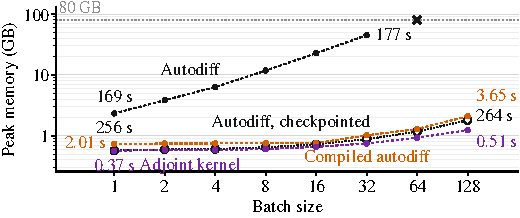
\includegraphics[width=\columnwidth]{figures/benchmark-dots-label.pdf}
 \caption{Peak memory and time per step at the first and last batch sizes.}
 \label{fig:benchmark}
\end{figure}

\bibliographystyle{IEEEtran}
{\footnotesize\bibliography{references}}
\end{sloppy}
\end{document}
